%!TEX root = ../thesis.tex

\chapter{Implementation}
\label{ch:implementation}

Text text

\section{Existing implementation}

As we have already mentioned, an implementation has already been attempted for this project.
Before we can begin with a new one, we first have to decide which parts of the existing one we want to use, and which to discard.
These parts are summarized in this section.

\subsection{SCM Expansion}

The SCM package has been expanded for GitHub to support the following functions:

\begin{itemize}
    \item CreateIssue   - creates an issue on a repository.
    \item EditRepoIssue - edits an issue on a repository.
    \item GetRepoIssue  - retrieves an issue based on issue number and repository.
    \item GetRepoIssues - retrieves all issues from a repository.
\end{itemize}

CreateIssue and EditRepoIssue would prove useful, and are used with only minor adjustments to them.
The two other functions, centered around retrieving issues were not needed, but still used in earlier parts of the project when testing.

\subsection{Logic}

A lot of existing code was intended to handle the logic around managing tasks. 
In short, this code was meant to do determine when to create, edit or delete issues on GitHub.
The code did however not accomplish this in a functional manner.
This lead to the dilemma of whether we should continue developing this faulty code, or simply start anew.
In the end, it was decided that any attempt to fix the existing logic code would be more time consuming and confusing, than simply starting fresh.

\subsection{Parsing Tasks}
\label{sec:parsing_tasks}

When a teacher pushes assignments to the \textit{tests} repository QuickFeed will run the function UpdateFromTestsRepo.
In short, this function fetches the files of \textit{tests}, loops through them, and uses their contents to create or update the data records of all course assignments.
Added as a part of this process, was code to also fetch task files in the repository, and use their contents to create a task data object.

To support this, all \textit{task-*.md} files are expected to conform to a standard format.
The first line should start with the character sequence "\# <task title>", followed by by two new line characters.
Any following text will be treated as the task body or description.

Using this format, the function newTask creates a task data object from any task file.

\lstinputlisting[caption={Function that creates a task object from markdown content}, language=Golang, firstline=25, lastline=40]{code/tasks.go}

Going forward, the general approach to parsing and creating tasks is left as it is, with only minor changes to the existing code.

\section{Managing Tasks and Issues}

Having looked at what existing code we decided to keep, we continue by exploring the part of the project that was implemented first, how to manage tasks and issues.
Building on what is described in section \ref{sec:tasks_and_github_issues}, this section describes the actual implementation process.

Moving forward in this chapter, we make the following distinction between found tasks and assignments, and existing tasks and assignments.
Found tasks and assignments are data objects created from the contents within the \textit{tests} repository.
Existing tasks and assignments are data-objects based on data records that we retrieve from the database.

\subsection{Data structures}

Two new messages are defined in the ag.proto file: \textbf{Task} and \textbf{Issue}.
These are used to generate the data structures that we use throughout the rest of the project.

\textbf{Task} is defined as follows:

\lstinputlisting[caption={Task message}, firstline=185, lastline=193]{code/ag.proto}

Every task is associated with one assignment via the \textit{assignmentID} field.

For assignments, \textit{order} is a number used to determine the order in which assignments are represented in a course.
Tracking the order of the assignment a task came from, allows us to associate tasks and assignments without explicitly knowing the assignment ID, so long as our scope is limited to just a single course.
A feature that will prove necessary.

The \textit{name} field is used to associate tasks found on GitHub, with the ones stored in the database.
If a task file with the name task-hello\_world.md is found within assignment1, then its corresponding name will be assignment1/hello\_world.
This name is set when the task itself is parsed, as described in section \ref{sec:parsing_tasks}.

\textbf{Issue} is defined as follows:

\lstinputlisting[caption={Issue message}, firstline=195, lastline=200]{code/ag.proto}

We see that every issue holds an association to the task that was used to create it, as well as the repository it was created on.

The \textit{issueNumber} field represents the issue number GitHub will assign the issue on its creation.

As it will become important in the next section, we will also mention that a modification was made to the existing message \textbf{Assignment}.

\lstinputlisting[caption={Assignment message}, firstline=168, lastline=183]{code/ag.proto}

On line 14 on the above code we see that the message has repeated tasks.
When we compile it, the resulting data structure can hold a slice of tasks.

\subsection{Main Logic}

As mentioned in section \ref{sec:parsing_tasks}, UpdateFromTestsRepo is the function that is run when someone pushes to the \textit{tests} repository.
Since tasks and issues need to be synchronized every time this happens, all logic for doing so will happen here.

More specifically, we create the function handleTasks that handles all logic relating to tasks.
It is supplied with every found assignment, and their respective found tasks, as an argument.
The function itself is run at the end of UpdateFromTestsRepo.

\lstinputlisting[caption={The function handleTasks, responsible for all task related logic}, language=Golang, firstline=64, lastline=95]{code/tasks.go}

The logic contained in this function will be explained in the following sections.

\subsection{Synchronizing Tasks}

When teachers create, edit, and delete tasks, we must make sure that the same happens in QuickFeed's internal database.
To accomplish this, we created the database method SynchronizeAssignmentTasks to synchronize tasks correctly.
This method is run at the start of handleTasks, and can be summarized in the following chart.

\begin{figure}[ht]
    \centering
    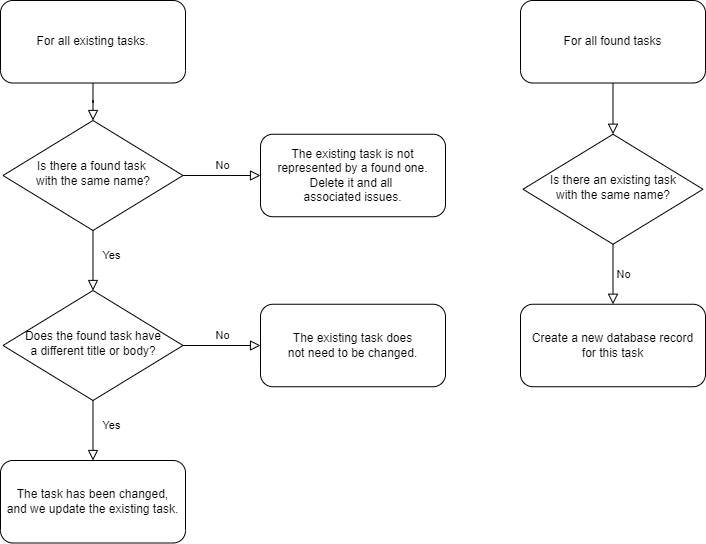
\includegraphics[width=\textwidth]{photos/synchronize-tasks-flow-chart.png}
    \caption{Flow chart describing how tasks are synchronized}
    \label{fig:synchronize-tasks-flow-chart}
\end{figure}

To support this logic, SynchronizeAssignmentTasks utilizes Go's built in maps to map tasks by both assignment order and name.
When looping through all existing assignments and then their respective existing tasks, we can use this mapping to perform all checks described in the chart above.

\lstinputlisting[caption={Logic performed in SynchronizeAssignmentTasks}, language=Golang, firstline=41, lastline=76]{code/gormdb_tasks.go}

SynchronizeAssignmentTasks also returns the tasks it has created or updated, which will be important when synchronizing issues.

\subsection{Synchronizing Issues}

\section{Tests}

Maybe maybe